\documentclass{article}
\usepackage{graphicx}
\usepackage{tikz}
\usepackage{geometry}
\usepackage{listings}
\usepackage{xcolor}
\usetikzlibrary{shapes.geometric, arrows, positioning}

\title{TCP File Transfer System Design}
\author{
Nguyen Quoc Khanh (22bi13210)
Pham Tien Dat (22bi13080)
Bui Thanh Vinh (22bi13469)
Pham Duc Gia Hien (22bi13155)}
\date{20/11/2024}

\begin{document}

\section*{TCP-Based File Transfer Protocol}

This report presents the design, organization, and implementation of a TCP-based file transfer system. The primary goal is to explore the fundamental principles of network programming and distributed systems by developing a simple yet functional file transfer protocol.

\subsection*{1. Protocol Steps}

The protocol consists of three main phases:

\begin{enumerate}
    \item \textbf{Connection Establishment:}
    \begin{itemize}
        \item The client initiates a TCP connection to the server using the three-way handshake:
        \begin{enumerate}
            \item The client sends a SYN packet to the server.
            \item The server responds with a SYN-ACK packet.
            \item The client sends an ACK packet, establishing the connection.
        \end{enumerate}
    \end{itemize}

    \item \textbf{Data Transmission:}
    \begin{itemize}
        \item The client reads the file in chunks of predefined size (e.g., 1024 bytes) and sends each chunk to the server.
        \item The server receives these chunks and writes them to a file.
    \end{itemize}

    \item \textbf{Connection Termination:}
    \begin{itemize}
        \item Once the file transfer is complete, the client closes the connection.
        \item The server finalizes the operation and saves the file.
    \end{itemize}
\end{enumerate}

\maketitle

\section{System Architecture}
The TCP file transfer system is implemented using Python's socket programming, consisting of two primary components: a client (\texttt{echo-client.py}) and a server (\texttt{echo-server.py}). The system enables file transmission over a local network using TCP/IP protocol.

\begin{figure}[h]
    \centering
    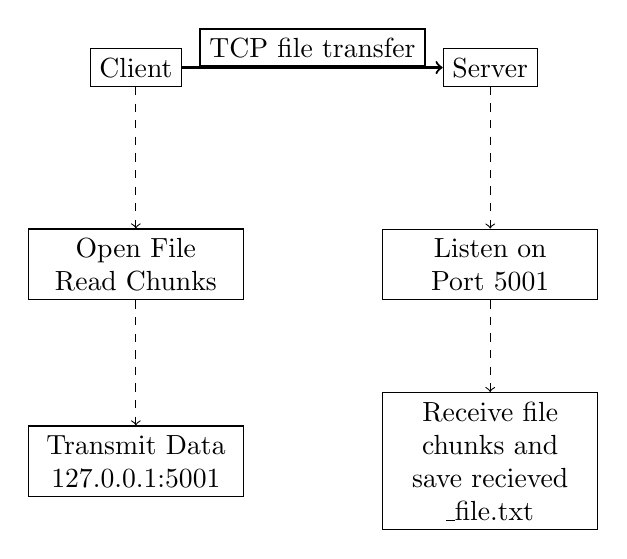
\begin{tikzpicture}[node distance=1.5cm, every node/.style={draw, rectangle}]
        % Nodes
        \node (client) {Client};
        \node[right of=client, xshift=3cm] (server) {Server};
        
        % Connection arrow
        \draw[thick, ->] (client) -- node[midway, above] {TCP file transfer} (server);
        
        % Client side steps
        \node[below of=client, yshift=-1cm, text width=2.5cm, align=center] (open) {Open File\\ Read Chunks};
        \node[below of=open, yshift=-1cm, text width=2.5cm, align=center] (transmit) {Transmit Data\\ 127.0.0.1:5001};
        
        % Server side steps
        \node[below of=server, yshift=-1cm, text width=2.5cm, align=center] (listen) {Listen on\\ Port 5001};
        \node[below of=listen, yshift=-1cm, text width=2.5cm, align=center] (receive) {Receive file chunks and\\save recieved \_file.txt};
        
        % Connecting lines
        \draw[dashed, ->] (client) -- (open);
        \draw[dashed, ->] (open) -- (transmit);
        \draw[dashed, ->] (server) -- (listen);
        \draw[dashed, ->] (listen) -- (receive);
    \end{tikzpicture}
    \caption{TCP File Transfer System Communication Flow}
    \label{fig:file_transfer_flow}
    \end{figure}

\section{Implementation Details}
\subsection{Client-Side (\texttt{echo-client.py})}
\begin{itemize}
    \item Uses \texttt{socket.socket()} to create a TCP connection
    \item Connects to server at \texttt{127.0.0.1:5001}
    \item Reads file in \texttt{1024} byte chunks
    \item Sends file data using \texttt{sendall()} method
\end{itemize}

\subsection{Server-Side (\texttt{echo-server.py})}
\begin{itemize}
    \item Binds to localhost on port \texttt{5001}
    \item Accepts incoming client connection
    \item Receives file chunks and reconstructs file
    \item Saves received file as \texttt{received\_file.txt}
\end{itemize}

\section{Conclusion}
The implemented system provides a simple, robust mechanism for transferring files using TCP sockets, demonstrating basic principles of network programming and distributed systems.


\subsection*{Figure of the File Transfer Process}

\begin{center}
\begin{tikzpicture}[node distance=2cm]

% Nodes
\node (client) [startstop] {Client};
\node (server) [startstop, right of=client, xshift=6cm] {Server};

% Client side nodes
\node (readfile) [process, below of=client] {Open File, Read Chunks};
\node (senddata) [process, below of=readfile] {Transmit Data to 127.0.0.1:5001};

% Server side nodes
\node (listen) [process, below of=server] {Listen on Port 5001};
\node (receive) [process, below of=listen] {Receive File Chunks \\ and Save as file.txt};

% Arrows
\draw [arrow] (client) -- (readfile);
\draw [arrow] (readfile) -- (senddata);

\draw [arrow] (server) -- (listen);
\draw [arrow] (listen) -- (receive);

% Connecting client and server
\draw [arrow, dashed] (senddata.east) -- ++(2cm,0) |- (listen.west);

\end{tikzpicture}
\end{center}

\section*{Conclusion}

The described protocol and its implementation demonstrate a simple and reliable method for transferring files over a TCP connection. By breaking the file into chunks, the system ensures efficient handling of data, and the use of Python's \texttt{socket} module provides robust network communication.

\subsection*{3. Implementation of the file transfer and Code Snippet}

The implementation of the protocol consists of a client and a server program written in Python. Below are the code snippets for both.

\subsubsection*{Client-Side Implementation}

The client reads the file and sends it to the server in chunks.

\begin{lstlisting}[caption=Client-Side File Transfer, label=lst:client]
import socket

SERVER_HOST = '127.0.0.1'  # Server address
SERVER_PORT = 5001         # Server port
BUFFER_SIZE = 1024         # Chunk size for reading and sending

def send_file(file_path):
    # Create a TCP socket
    client_socket = socket.socket(socket.AF_INET, socket.SOCK_STREAM)
    client_socket.connect((SERVER_HOST, SERVER_PORT))  # Connect to the server
    print(f"Connected to server {SERVER_HOST}:{SERVER_PORT}")

    # Open the file and send its contents in chunks
    with open(file_path, 'rb') as file:
        while (chunk := file.read(BUFFER_SIZE)):  # Read the file in 1024-byte chunks
            client_socket.sendall(chunk)         # Send the chunk to the server
    
    print("File transfer complete.")
    client_socket.close()  # Close the connection
\end{lstlisting}

\subsubsection*{Server-Side Implementation}

The server receives the file data from the client and writes it to a local file. \\

\begin{lstlisting}[caption=Server-Side File Transfer, label=lst:server]
import socket

SERVER_HOST = '127.0.0.1'  # Listen on all available interfaces
SERVER_PORT = 5001         # Port to listen on
BUFFER_SIZE = 1024         # Chunk size for receiving data

def start_server():
    # Create a TCP socket
    server_socket = socket.socket(socket.AF_INET, socket.SOCK_STREAM)
    server_socket.bind((SERVER_HOST, SERVER_PORT))
    server_socket.listen(1)  # Listen for a single connection
    print(f"Server listening on {SERVER_HOST}:{SERVER_PORT}")

    # Accept client connection
    conn, addr = server_socket.accept()
    print(f"Connection established with {addr}")

    # Open a file to save the received data
    with open("received_file.txt", "wb") as file:
        while True:
            # Receive file chunks
            data = conn.recv(BUFFER_SIZE)
            if not data:  # End of file
                break
            file.write(data)  # Write the received chunk to the file
    
    print("File transfer complete. File saved as 'received_file.txt'")
    conn.close()
    server_socket.close()
\end{lstlisting}

\end{document}
